\chapter{DESKRIPSI SISTEM}

\section{Deskripsi Umum}

Lorem ipsum dolor sit amet, consectetur adipiscing elit. Proin interdum in est sed imperdiet. Praesent nec mauris finibus, luctus risus ut, suscipit urna. Class aptent taciti sociosqu ad litora torquent per conubia nostra, per inceptos himenaeos. Nulla ut nulla ut dolor efficitur cursus. Pellentesque habitant morbi tristique senectus et netus et malesuada fames ac turpis egestas.

Quisque venenatis sapien sed vulputate tempus. Fusce sagittis enim eu dui vestibulum posuere. Orci varius natoque penatibus et magnis dis parturient montes, nascetur ridiculus mus. Suspendisse luctus metus ipsum.

\section{Spesifikasi Sistem}
\subsection{Perangkat Lunak}
\begin{table}[ht!]
    \centering
    \begin{tabular}{|l|l|l|l|}
        \hline
        Sitem Operasi                   & MacOS X Ventura    \\ \hline
        \multirow{2}{*}{\textit{Tools}} & XCode              \\ \cline{2-2}
                                        & Visual Studio Code \\ \hline
    \end{tabular}
    \caption{Perangkat Lunak}
    \label{tab:softwareUsed}
\end{table}

\subsection{Perangkat Keras}
\begin{table}[ht!]
    \centering
    \begin{tabular}{|l|l|l|l|}
        \hline
        \textit{Proccessor} & Intel(R) Core i9 \\ \hline
        RAM                 & 32GB             \\ \hline
        SSD                 & 500GB            \\ \hline
    \end{tabular}
    \caption{Perangkat Keras}
    \label{tab:hardwareUsed}
\end{table}

\subsection{Pemrograman}
\begin{table}[ht!]
    \centering
    \begin{tabular}{|l|l|l|l|}
        \hline
        Bahasa Pemrograman                  & Swift            \\ \hline
        \multirow{4}{*}{\textit{Framework}} & SwiftUI          \\ \cline{2-2}
                                            & UIKit            \\ \cline{2-2}
                                            & Core Data        \\ \cline{2-2}
                                            & AV Foundation    \\ \cline{2-2}
                                            & Natural Language \\ \hline
        \multirow{4}{*}{\textit{Library}}   & Native Base      \\ \cline{2-2}
                                            & Firebase Core    \\ \cline{2-2}
                                            & Google MLKit     \\ \hline
        \textit{Versioning control system}  & Git \& GitHub    \\ \hline
    \end{tabular}
    \caption{Perangkat Lunak}
    \label{tab:programmingLanguage}
\end{table}

\section{Perancangan Sistem}

\subsection{Use Case Diagram}

Quisque venenatis sapien sed vulputate tempus. Fusce sagittis enim eu dui vestibulum posuere. Orci varius natoque penatibus et magnis dis parturient montes, nascetur ridiculus mus.
\begin{figure}[H]
    \centering
    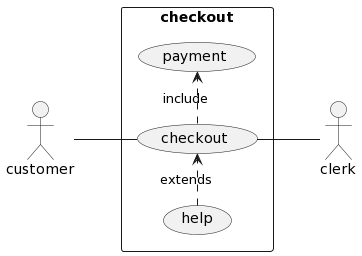
\includegraphics[width=10cm]{assets/pics/dummy-use-case-diagram.png}
    \caption{Use Case Diagram Aplikasi ABCD}
    \label{fig:usecaseDiagram}
\end{figure}

Fusce sagittis enim eu dui vestibulum posuere. Orci varius natoque penatibus et magnis dis parturient montes, nascetur ridiculus mus.

\subsection{Class Diagram}
Quisque venenatis sapien sed vulputate tempus. Fusce sagittis enim eu dui vestibulum posuere. Orci varius natoque penatibus et magnis dis parturient montes, nascetur ridiculus mus.

\begin{figure}[H]
    \centering
    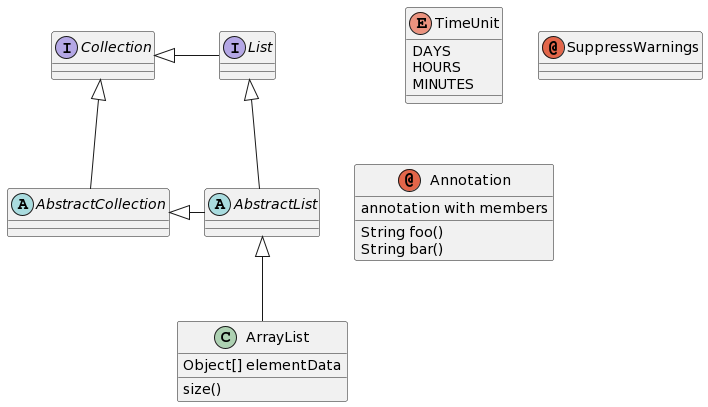
\includegraphics[width=10cm]{assets/pics/dummy-class-diagram.png}
    \caption{Class Diagram Aplikasi ABCD}
    \label{fig:classDiagram}
\end{figure}

Fusce sagittis enim eu dui vestibulum posuere. Orci varius natoque penatibus et magnis dis parturient montes, nascetur ridiculus mus.

\subsection{Activity Diagram}
Quisque venenatis sapien sed vulputate tempus. Fusce sagittis enim eu dui vestibulum posuere. Orci varius natoque penatibus et magnis dis parturient montes, nascetur ridiculus mus.
\subsubsection{Activity Diagram A}
\begin{figure}[H]
    \centering
    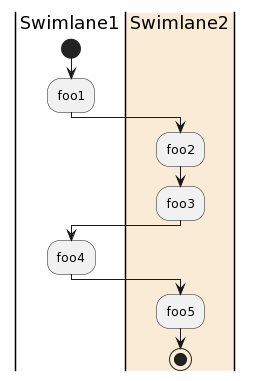
\includegraphics[width=10cm]{assets/pics/dummy-activity-diagram.png}
    \caption{Activity Diagram A}
    \label{fig:activityDiagramA}
\end{figure}

Quisque venenatis sapien sed vulputate tempus. Fusce sagittis enim eu dui vestibulum posuere. Orci varius natoque penatibus et magnis dis parturient montes, nascetur ridiculus mus.

\subsubsection{Activity Diagram B}
\begin{figure}[H]
    \centering
    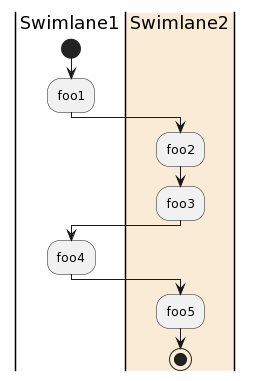
\includegraphics[width=10cm]{assets/pics/dummy-activity-diagram.png}
    \caption{Activity Diagram B}
    \label{fig:activityDiagramB}
\end{figure}

Quisque venenatis sapien sed vulputate tempus. Fusce sagittis enim eu dui vestibulum posuere. Orci varius natoque penatibus et magnis dis parturient montes, nascetur ridiculus mus.

\subsection{Sequence Diagram}
Quisque venenatis sapien sed vulputate tempus. Fusce sagittis enim eu dui vestibulum posuere. Orci varius natoque penatibus et magnis dis parturient montes, nascetur ridiculus mus.
\subsubsection{Sequence Diagram A}
\begin{figure}[H]
    \centering
    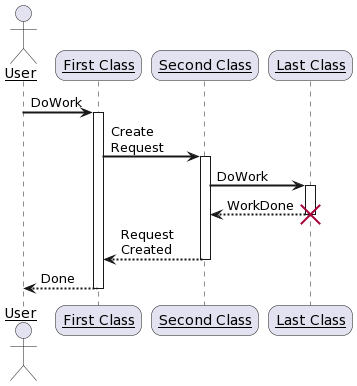
\includegraphics[width=10cm]{assets/pics/dummy-sequence-diagram.png}
    \caption{Sequence Diagram A}
    \label{fig:sequenceDiagramA}
\end{figure}

Quisque venenatis sapien sed vulputate tempus. Fusce sagittis enim eu dui vestibulum posuere. Orci varius natoque penatibus et magnis dis parturient montes, nascetur ridiculus mus.

\subsubsection{Sequence Diagram B}
\begin{figure}[H]
    \centering
    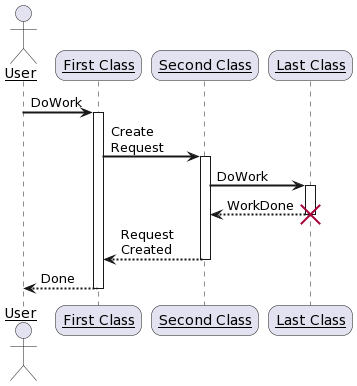
\includegraphics[width=10cm]{assets/pics/dummy-sequence-diagram.png}
    \caption{Sequence Diagram B}
    \label{fig:sequenceDiagramB}
\end{figure}

Quisque venenatis sapien sed vulputate tempus. Fusce sagittis enim eu dui vestibulum posuere. Orci varius natoque penatibus et magnis dis parturient montes, nascetur ridiculus mus.

\subsection{Tabel Relasi}
Quisque venenatis sapien sed vulputate tempus. Fusce sagittis enim eu dui vestibulum posuere. Orci varius natoque penatibus et magnis dis parturient montes, nascetur ridiculus mus.

\subsubsection{Tabel A}
Quisque venenatis sapien sed vulputate tempus. Fusce sagittis enim eu dui vestibulum posuere.

\begin{table}[ht!]
    \centering
    \begin{tabular}{|l|l|l|l|}
        \hline
        \textbf{Nama\_\textit{Field}} & \textbf{\textit{Type}} & \textbf{\textit{Null}} & \textbf{\textit{Default}} \\ \hline
        ID                            & -                      & -                      & -                         \\ \hline
        name                          & -                      & -                      & -                         \\ \hline
        email                         & -                      & -                      & -                         \\ \hline
        password                      & -                      & -                      & -                         \\ \hline
        is\_active                    & -                      & -                      & -                         \\ \hline
    \end{tabular}
    \caption{Table A}
    \label{tab:relationTableA}
\end{table}

\subsubsection{Tabel B}
Orci varius natoque penatibus et magnis dis parturient montes, nascetur ridiculus mus. Orci varius natoque penatibus et magnis dis parturient montes, nascetur ridiculus mus.
\begin{table}[ht!]
    \centering
    \begin{tabular}{|l|l|l|l|}
        \hline
        \textbf{Nama\_\textit{Field}} & \textbf{\textit{Type}} & \textbf{\textit{Null}} & \textbf{\textit{Default}} \\ \hline
        ID                            & -                      & -                      & -                         \\ \hline
        name                          & -                      & -                      & -                         \\ \hline
        email                         & -                      & -                      & -                         \\ \hline
        password                      & -                      & -                      & -                         \\ \hline
        is\_active                    & -                      & -                      & -                         \\ \hline
    \end{tabular}
    \caption{Table B}
    \label{tab:relationTableB}
\end{table}